\subsubsection{Command} % (fold)
\label{ssub:command}

Incapsula una richiesta, un azione o una transazione in un oggetto, permettendo
di parametrizzare oggetti con diverse richieste, accodare o \emph{loggare}
richieste, e supportare operazioni annullabili (\frgnword{undo}.)

Il pattern command risponde alla necessità di creare richieste a oggetti senza
conoscere nulla l'operazione richiesta o il ricevente della richiesta.

\paragraph{Applicabilità} % (fold)
\label{par:applicabilit_}

\begin{itemize}
  \item Parametrizzare oggetti con azioni da eseguire (si pensi ad un menuitem,
    al quale un client esterno può assegnare l'azione da svolgere al click
    dell'utente.) Command rappresenta l'alternativa \frgnword{object-oriented}
    delle callback procedurali;
  \item Specificare, accodare e eseguire richieste in tempi differenti;
  \item Supportare operazioni reversibili (\frgnword{undo}).
    L'operazione execute() dell'oggetto Command può memorizzare stato per
    annullare i suoi effetti all'interno del Command stesso, e offrire un metodo
    unexecute();
  \item Supportare il \frgnword{logging} dei cambiamenti in modo da poterli
    riapplicare in caso di crash del sistema;
  \item Supportare transazioni, operazioni ad alto livello costruite su
    operazioni primitive.
\end{itemize}

\begin{figure}
  \centering
  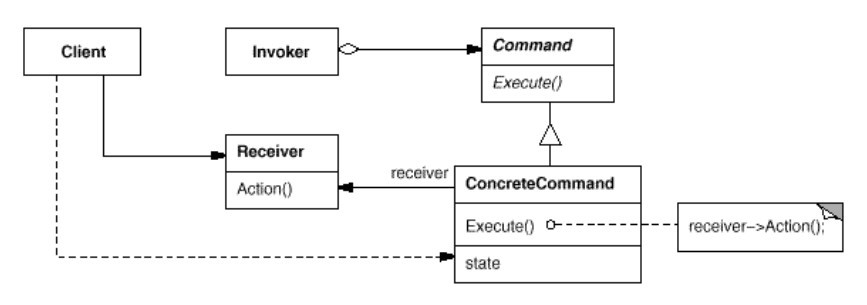
\includegraphics[scale=0.5]{imgs/command}
  \caption{Diagramma delle classi del pattern Command}
\end{figure}

\paragraph{Collaborazioni} % (fold)
\label{par:collaborazioni}

\begin{itemize}
  \item Il client crea un oggetto command concreto e specifica il suo receiver;
  \item Un oggetto invoker memorizza l'oggetto command concreto;
  \item L'invoker issues una richiesta chiamando il metodo execute del command.
  \item Il command concreto invoca operazioni sul receiver per portare a termine
  la richiesta.
\end{itemize}

\paragraph{Conseguenze} % (fold)
\label{par:conseguenze}

\begin{itemize}
  \item Command disaccoppia l'oggetto che invoca l'operazione da quello che la
  esegue;
  \item I command sono \frgnword{first-class objects}, e pertanto sono
  manipolabili come tali;
  \item Più command possono essere assemblati in command composti;
  \item L'aggiunta di nuovi command è semplice poichè non è necessaria la
  modifica di classi già esistenti.
\end{itemize}
